\documentclass[12pt]{article}
\usepackage[a4paper,fancysections,titlepage]{polytechnique}
\usepackage{amsmath,bm,empheq,graphicx,hyperref,siunitx,subcaption,upgreek,xcolor}
\usepackage[italicdiff]{physics}
\usepackage[justification=centering]{caption}
\usepackage{indentfirst}

\hypersetup{colorlinks=true, urlcolor=cyan}
\newcommand{\angstrom}{\textup{\AA}}
\newcommand{\ddfrac}[2]{{\displaystyle\frac{\displaystyle #1}{\displaystyle #2}}}

\title{Quantum Criticallity in Cuprate Superconductors: PRL Report}
\author{Matéo Rivera, Saleh Shamloo Ahmadi\\Supervisor: Gaël Grissonnanche}
\date{March 17, 2025}

\begin{document}
\maketitle
\section{Introduction \& Problem Statement}

We carried out our project under the supervision of Prof. Gaël Grissonnanche in his group at \textit{Laboratoire des Solides Irradiés} (Laboratory for Irradiated Solids, LSI). 
The LSI is a joint research unit of CNRS, CEA and École polytechnique, hosted on École polytechnique's campus.
It notably hosts an electron irradiator used by researchers worldwide to add controlled disorder to materials ranging from cements in nuclear power plants to satellite photovoltaics and quantum materials.

The group's research focuses on the study of quantum materials under extreme temperature and magnetic field conditions. 
Their laboratory consists of two refrigerators that can go from room temperature to near absolute zero ($\sim 10$ millikelvin).
These refrigerators are equipped with a large superconducting magnet, 
each capable of operating at up to 14 teslas.

As our project was numerical (leveraging published experimental data),  
we didn't carry out experiments using this equipment and were supervised by Prof. Grissonnanche only. 


\subsection{Cuprates: High temperature superconductors}
\begin{figure}
    \centering
    \begin{subfigure}{0.37\textwidth}
        \centering
        \includegraphics[width=\textwidth]{figures/cuprate_structure}
        \caption{Crystal structure of a Cuprate (YBCO)}
        \label{fig:cuprate_structure}
    \end{subfigure}\hfill
    \begin{subfigure}{0.5\textwidth}
        \centering
        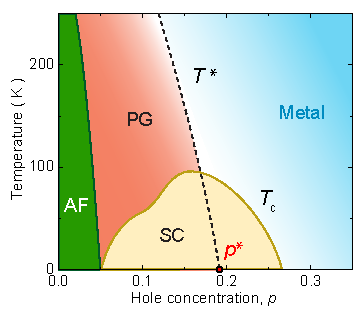
\includegraphics[width=\textwidth]{figures/phase_diagram}
        \caption{Phase diagram of cuprates}
        \label{fig:phase_diagram}
    \end{subfigure}
    \caption{Physical description of cuprates. (a) shows the provskite structure of a cuprate,
    and (b) shows the different phases of cuprates in a phase diagram. $p^*$ marks the hypothesised
    quantum critical point. AF, PG, and SC stand for Antiferromagnetic, Pseudogap, and
    Superconducting phases respectively.}
\end{figure}

Cuprates are a class of superconductors with high critical temperature that have been subject
to intense research since their discovery in 1986. They exhibit rich physical behavior, specially
in their various phases.

The crystal structure of cuprates is a perovskite structure, with a copper-oxygen plane
($\mathrm{CuO}_2$) as the main conducting layer. This structure is shown in Figure
\ref{fig:cuprate_structure}. You can think of cuprates as a stack of different conducting layers,
so the electronic properties of cuprates are mainly 2D. However, the interlayer coupling is
non-negligible, and the 3D nature of cuprates is important for their physical properties.

The phase diagram of cuprates is shown in Figure \ref{fig:phase_diagram}. The main phases of
cuprates are the Antiferromagnetic (AF) phase, the metallic phase, the Pseudogap (PG) phase,
the Superconducting (SC) phase. The metallic phase itself can be split into a strange metal
phase (with anamolous electronic scattering properties) and a normal metal phase (with
well-described conductivity, using Fermi liquid theory). There is also a hypothesised point in the
phase diagram called the quantum critical point, marked as $p^*$ in the figure.

\subsection{Origin of Cuprate Superconductivity: The Quantum Critical Point}
\begin{figure}
    \centering
    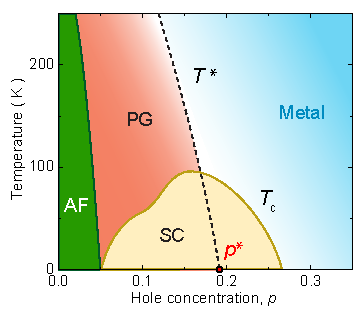
\includegraphics[width=0.5\textwidth]{figures/phase_diagram}
    \caption{Phase diagram of Cuprates. $p^*$ marks the QCP.}
    \label{fig:phase_diagram}
\end{figure}

The origin of high-temperature superconductivity in Cuprates is still the subject of intense
research and debate, but a possible explanation has to do with the Quantum Critical Point (QCP).
The QCP is a point in the phase diagram of a material where there is a phase transition at zero
temperature. This phase transition is driven by quantum effects, hence the name. In the case of
Cuprates, this is a critical doping level, usually denoted by $p_c$ or $p^*$. The actual existence
of a QCP for Cuprates is still a matter of debate and it is the subject of this project.

In their 2019 paper, Michon et al. \cite{michon2019} used secific heat measurements to
show the existence of the QCP. The effective mass of the charge carriers is expected to diverge at
the QCP, and the effective mass is proportional to $C/T$ where $C$ is the specific heat attributed
to the charge carriers and $T$ is the temperature. So, to probe the QCP, Michon et al. measured
the specific heat at very low temperatures (1 to 2 K) and extrapolated to zero temperature. More
specifically, they show
\begin{equation}
    \frac{C(T)}{T} = \gamma + \beta T^2.
\end{equation}
They found $\gamma$ peaks at the critical doping level, which is the signature of the QCP.
\begin{figure}
    \centering
    \begin{subfigure}{0.48\textwidth}
        \centering
        \includegraphics[width=\textwidth]{figures/michon}
        \caption{Measurements of Michon et al. showing a peak in $C/T$ which signifies the existence
            of a QCP.}
        \label{fig:michon}
    \end{subfigure}\hfill
    \begin{subfigure}{0.48\textwidth}
        \centering
        \includegraphics[width=\textwidth]{figures/legros}
        \caption{Measurements of Legros et al. drawn onto the measurements from Michon et al.,
            showing no peak in the cyclotron mass.}
        \label{fig:michon}
    \end{subfigure}
    \caption{Comparison of the measurements of Michon et al. and Legros et al.}
    \label{fig:comparison}
\end{figure}

\subsection{Evidence against the QCP: Optical Conductivity}
In their 2022 paper, Legros et al. \cite{legros2022} instead used optical conductivity to
probe the QCP. To do so, the first measured the optical conductivity of LSCO cuprates in various
fields. Then, they fitted a model for the conductivity called the Drude formula to the data. The
Drude formula is a simple classical model that has been used for a long time in condensed matter
physics to model conductivity. Next, they extracted the cyclotron mass from the parameters of the
fit. Finally, they extracted the cyclotron mass from the parameters of the fit. To do so, they
calculated the cyclotron frequency in different magnetic fields and found the mass by fitting a
linear relation between the cyclotron frequency and the magnetic field;
\begin{equation}
    \omega_c = \frac{eB}{m_c}.
\end{equation}
They argue the cyclotron mass is the same as the effective mass of the charge carriers
($m_c \sim m^*$).

At the end of all the analysis, Legros et al. found that the cyclotron mass does not peak
at the critical doping level and simply increases with doping. This is in contradiction with the
results of Michon et al. and suggests that there is no QCP in Cuprates.

We believe, however, that their data analysis is problematic, because of the use of the Drude
formula. Eventhough the Drude formula is derived using classical physics, it is highly effective for
analysing the conductivity of materials, which emerges from the collective quantum behavior of the
electrons. But, this is only the case when the material has roughly isotropic electronic properties
(more precisely, the Fermi surface needs to be approximately isotropic). This is not true for
Cuprates, which have highly anisotropic electronic properties. Also, the effective mass of the
charge carriers is not necessarily the same as the cyclotron mass, but we only focus on the former
issue in this project.

\subsection{How to resolve the contradiction?}
In light of these contradicting conclusions, our project seeks to investigate a possible solution.
On the one hand, Michon et al.\cite{michon2019} probe criticality directly: 
that is, they look for a thermodynamic phase transition using a heat capacity measurement.

On the other hand, Legros et al.\cite{legros2022} probe it indirectly using a measurement of optical conductivity: 
$m_c$ is a parameter resulting from a fit of the experimental data. 
Thus, any results are dependent on the theoretical model chosen to fit the data.

An alternative to the Drude model used by Legros et al.\cite{legros2022} is the Chambers formula, 
derived from Boltzmann transport theory.  While the Drude model is derived for a
free electron (meaning it has isotropic transport properties), 
Boltzmann transport takes into account such anisotropy and more of the microscopic details of the
material.  This is particularly interesting for the study of cuprate high temperature
superconductors, where anisotropy is suspected to be of paramount importance.


\subsection{Goals}
During our project, we gradually set and met the following goals. In particular, we succeeded to: 
\begin{itemize}
	\item develop a tool to extract data from graphs published in the literature;
	\item reproduce the fitting results of the papers we extracted the data from;
	\item develop a tool to calculate a better model (Chambers' formula) by adapting existing code used for other experiments;
	\item analytically compare the two models (Drude and Chambers') and show that the latter reduces to the former under a 'free electron' hypothesis;
	\item validate the new numerical method by comparing calculated numerical results in the 'free electron' hypothesis with the Drude model;
	\item develop a fitting tool leveraging the new code, existing packages;
	\item qualitatively analyze (explore) the parameter space to prepare fitting;
	\item perform the fits and find the best fitting protocol on one data from one doping level.
	\item repeat the fitting on data from other doping levels.
	\item extract the effective mass from the fitting results.
	\item compare the results with the literature.
\end{itemize}
Due to a lack of time, we were not able to:
\begin{itemize}
	\item do rigorous error analysis;
	\item make a more complex model for lower doping levels;
\end{itemize}

\section{Methods}
\subsection{What is optical conductivity ?}
% Explain what it is and why we use it
The physical quantity of interest in this experiment is optical conductivity, 
the principle of which we will briefly explain.

Conductivity is often measured in static conditions : 
that is, for a constant or slowly varying applied electric fields. 
However, as for many physical systems, 
the dynamic response of the system is different from the static one. 

This dynamic response, 
that is the conductivity of a material under an applied electric field at a given frequency $\omega$, 
is precisely the optical conductivity $\sigma{\omega}$. 
Here, because we're talking about periodic excitations, this complex conductivity relates the amplitude and phase of current density to those of the applied electric field. \\

Optical conductivity is a powerful probe into the electronic properties of the examined material, 
giving a better insight than DC conductivity alone. 
Moreover, as is done in Legros et al., 
it is possible to apply an external magnetic field to the sample. 
This yields interesting behaviours such as Angle Dependent Magnetoresistance (ADMR) 
or the results of the experiment at hand. \\

% Touch on the experimental setup
There are several experimental setups used to measure optical conductivity. 
While in principle, we can probe any frequency domain, 
we are in practice interested in the optical frequencies. 
In this case, there are two main categories of experiments that can be carried out : 
transmission and reflection. 


Legros et al. chose a transmission setup through a thin film ($\sim 10$ nm, 10-100 layers) as their method. 
The full experimental setup is not without challenges but is not directly relevant to our study. 
However, we can note that since the electronic properties of cuprates are mainly 2D 
(owing to their peroskite structure, as explained above), 
the use of thin films is not unreasonable 
and doesn't affect the relevance of the results for bulk materials.
\subsection{What are the hypotheses of the Drude model?}
As was stated previously, Legros et al. used the Drude model to analyze their data. 
This phenomenological model is common and of great use, but it assumes that we study 'free electrons' that only periodically get scattered with a scattering rate $\Gamma$, 
which is strictly speaking false for electrons in solids, 
where they interact with a periodic lattice.

We can translate this hypothesis in the language of condensed matter physics and band structure theory (which will simplify the comparison with Chambers' formula later). 
For a single electron, due to the periodicity of the lattice, 
we can define a quasi-momentum $\vb{k}$ which is a good quantum number and defines states with given energies. 
The filling of these levels according to Pauli's principle, by ascending energy, 
allows us to define a Fermi energy and corresponding Fermi surface 
which mostly determines the conduction properties of the material and can be, 
in many cases, determined experimentally and modelled theoretically.

What makes the Drude model useful is that in many cases, 
this Fermi surface can be approximated by a sphere, which yields the dispersion relation
$E(\vb{k}) = \frac{\hbar\vec{k}}{2m^*}$  that is formally equivalent to that of a free electron
(where $m^*$ is not necessarily $m_e$). The Drude model assumes a unique scattering rate
independent of $\vb{k}$.

In the end, Legros et al.\cite{legros2022} and others\cite{post2021} use the two-component Drude model with normal and superconducting carriers (in the presence of a magnetic field). 
In this model, the complex optical conductivity in the left/right circular polarization basis is given by
\begin{equation}
    \sigma_{ll/rr}(\omega) = i\epsilon_0\qty(
        \frac{\omega^2_{\mathrm{p,n}}}{\omega-\omega_c+i\Gamma}
        + \frac{\omega^2_{\mathrm{p,s}}}{\omega} - \omega(\epsilon_{\infty} - 1)),
\end{equation}
where $\omega$ is the frequency of the electromagnetic waves, $\epsilon_0$ is the vacuum
permittivity, and the adjustable parameters are
\begin{itemize}
    \item $\omega_{\mathrm{p,n}}$ and $\omega_{\mathrm{p,s}}$: plasma frequencies of the normal and
        superconducting charge carriers,
    \item $\omega_c = \frac{eB}{m_c}$: cyclotron frequency,
    \item $\Gamma$: scattering rate,
    \item $\epsilon_{\infty}$: high-frequency dielectric constant.
\end{itemize}
Left handed circular polarization is given by a negative $\omega$ and right handed by a positive $\omega$.

As stated in Legros et al. and other sources, 
the high-frequency dielectric constant ($\epsilon_\infty$) does not greatly improve the quality of the fit and its results, so it is set to 1.
Additionally, we can see here that in this model, the superconducting carriers only contribute to the imaginary part of $\sigma$. 
This ended up being relevant to inform our fitting choices in the end.

To extract the cyclotron mass from this model, one can fit the cyclotron frequency $\omega_c$ as a
function of the magnetic field $B$ and extract the mass from the slope of the linear fit, as the
relation between the two parameters is given by
\begin{equation}
    \omega_c = \frac{eB}{m_c},
\end{equation}
where $e$ is the elementary charge. This is the same approach used by Legros et al.\cite{legros2022}.

As mentioned before, this model breaks down for materials with highly anisotropic electronic properties
(i.e. highly anisotropic Fermi surfaces).

\subsection{Boltzmann Transport and Chambers Formula for Optical Conductivity}
The Boltzmann transport equation is a semi-classical model of flow 
which gives a more detailed model of the electronic properties of a material, 
since it accounts for the trajectories of the electrons in phase space. 
Chambers' formula thus describes the real electronic structure of the material, 
and can thus account for anisotropic scattering processes.

Using the Boltzmann equation, with a few reasonable assumptions, 
one can derive the Chambers formula for conductivity. 
The formula is usually applied for DC conductivity ($\sigma(\omega=0)$), 
but it can be generalized for optical conductivity too (see appendix \ref{sec:chambers}).
This model has been used successfully in the past to study the behavior of cuprates 
and make predictions about their physical properties\cite{grissonnanche2021, grissonnanche2024, fang2022, gourgout2022, ataei2022}, 
justifying its use here.

According to the Chambers formula for optical conductivity, 
the conductivity tensor in the cartesian basis is then given by :
\begin{equation}
	\sigma_{ab} = \frac{2e^2}{(2\pi)^d\hbar}\int_{\mathrm{FS}}\dd{\vb{k}}\hat{v}_a(\vb{k})
        \int_0^{\infty}\dd{t}v_b(\vb{k}(t))\exp{i\omega t
        - \int_0^t \frac{\mathop{dt'}}{\tau(\vb{k}(t'))}}
\end{equation}
where $\mathrm{FS}$ is the Fermi surface, $d$ is the number of dimensions of the system, $\vb{k}$ is the
wavevector, $\omega$ is the frequency of the electromagnetic waves, $v_b$ is the veclocity of the
charge carriers in the $b$ direction, $\hat{v}_a\equiv v_a/\abs{\vb{v}}$, and $\tau$ is the
relaxation time (inverse of the scattering rate). 

We can have an intuitive understanding of this formula. 
First, as we see here, we are only interested in the electrons that live on (or near, strictly speaking when at nonzero temperature) the Fermi surface as defined previously. 
Indeed, it is possible to show, as was mentioned above, that only they will meaningfully contribute to conduction. 
For any starting point $\vb{k}$ on the Fermi surface (first integral) with a given associated velocity in the $a$ component, 
we are interested the electron's velocity in the $b$ component along its trajectory (parametrised by $t$,  which can be time). 
The exponential terms account for the influence of the varying electrical field and the scattering rate of electron (that is not uniform in phase space). 
The magnetic field appears implicitly in the movement equations that define $\b{k}(t)$.

Thus, the formula reflects how, on average, electrons move in the $b$ direction when initially excited in the $a$ direction.


In order to evaluate the integral, we should then couple it with :
\begin{enumerate}
    \item a movement equation;
    \item a model for the scattering rate;
    \item the shape of the Fermi surface.
\end{enumerate}

In the following, 
we explain in more detail the different components and the methods of evaluating this formula.

\subsubsection{Movement Equation}
Since we are only interested in the first order response of the system to an electric field, we
can solve the movement equation with only a magnetic field. That is,
\begin{empheq}[left=\empheqlbrace]{align}
    \hbar\dv{\vb{k}}{t} &= e\vb{v}\times\vb{B}, \\
    \vb{v} &= \frac{1}{\hbar}\grad_{\vb{k}}\varepsilon(\vb{k}),
\end{empheq}
Where $\varepsilon$ is the energy of the charge carriers. The movement equation can be solved
numerically for a discretization of the Fermi surface (since the Chambers formula integral is
evaluated over the Fermi surface).

Here, note that the magnetic field $\vb{B}$ is always pointed along the $z$ direction for the data
we examined. However, our methods allow any direction for the magnetic field too.

\subsubsection{Scattering Rate}
Following Grissonnanche et al.\cite{grissonnanche2021}, we used a simple model for the scattering
rate, respecting the symmetry of the system. It is given by
\begin{equation}
    \frac{1}{\tau(\vb{k})} = \Gamma(\vb{k}) = \Gamma_0 + \Gamma_k\abs{\cos(2\varphi)}^\nu,
\end{equation}
where $\varphi$ is the angle between the wavevector and the $k_x$ axis and $\Gamma_0$, $\Gamma_k$,
and $\nu$ are adjustable parameters.

\subsubsection{Fermi Surface}
For the shape of the Fermi surface, we used a simple 3D tight-binding model for the Body centered
tetragonal crystal structure of LSCO, given by
\begin{equation}
\begin{aligned}
    \varepsilon(\vb{k}) = &-\mu - 2t(\cos(k_x a) + \cos(k_y a)) \\
        &- 4t'\cos(k_x a)\cos(k_y a) - 2t''(\cos(2k_x a) + \cos(2k_y a)) \\
        &- 2t_z\cos(k_x a / 2)\cos(k_y a / 2)\cos(k_z c / 2)[\cos(k_x a) - \cos(k_y a)]^2,
\end{aligned}
\end{equation}
where $\mu$ is the chemical potential, $t$, $t'$, and $t''$ are the first, second, and third
nearest-neighbor hopping parameters, $t_z$ is the interlayer hopping parameter,
$a=3.75\angstrom$ is the in-plane lattice constant, and $c/2=6.6\angstrom$ is the
$\mathrm{CuO_2}$ layer spacing. These parameters are derived experimentally from ARPES measurements\cite{horio2018}. \\

With this new formalism, we can now set out to use the Chambers formula to analyze the optical conductivity data produced by Legros et al.\cite{legros2022} to extract $m_c \approx m^*$.

Our goal is to see if our new $m_c$ still contradicts the effective mass obtained from specific heat. 


\section{Results}

\bibliographystyle{plain}
\bibliography{ref}

\end{document}